\section{Non-Metals and Their Compounds}

\begin{multicols}{2}


\section*{Chlorine}


\subsection{Preparation of Chlorine Gas}

\begin{center}
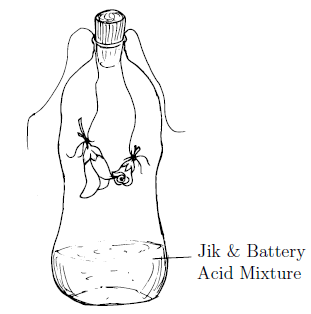
\includegraphics[width=0.4\textwidth]{./img/chlorine.png}
\end{center}

\begin{description*}
%\item[Subtopic:]{}
\item[Materials:]{Bleach, battery acid (5 M sulphuric acid), coloured 
flowers, string or thread,
bottle}
\item[Setup:]{Collect coloured 
flowers.
2. Cut about 30 cm of string for each 
flower and tie one to each flower.}
\item[Procedure:]{Put about 100 ml of bleach (e.g. Jik) in the bottle. Hang the 
flowers in the bottle using the strings. Tie the free end of
the string around the neck of the bottle. Add about 10 ml of battery acid to the bottle and quickly close the cap. Allow the bottle to sit for 5 minutes.}
\item[Hazards:]{This reaction produces chlorine, a poisonous gas. Perform this reaction
outside standing upwind. No students should attempt to
prepare chlorine outside of school.}
%\item[Questions:]{}
\item[Observations:]{The gas turns a greenish-yellow colour.}
\item[Theory:]{The chlorine gas will bleach the 
flowers in the
bottle. The bleaching action is due to the formation of hypochlorite ion,
formed when chlorine dissolves in water: $$
\ce{Cl2}_{(g)} + \ce{H2O} \longrightarrow \ce{HCl}_{(aq)} + \ce{HClO}_{(aq)} $$

$$\ce{HClO} + \mathrm{dye} \longrightarrow \mathrm{dye-O} + \ce{HCl}$$}
%\item[Applications:]{}
%\item[Notes:]{}
\end{description*}

%==================================================================================================%

\section*{Sulphur}


\subsection{Model of Sulphur $S_8$}

\begin{center}
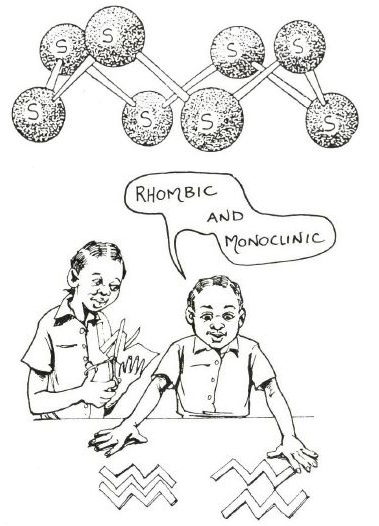
\includegraphics[width=0.4\textwidth]{./img/source/sulphur-model.jpg}
\end{center}

\begin{description*}
%\item[Subtopic:]{}
\item[Materials:]{Fruits/modeling clay/ugali, toothpicks}
%\item[Setup:]{}
\item[Procedure:]{(a) Use berries, fruits, modeling
clay spheres, balls of ugali, etc. for the sulphur atoms and
sticks for the bonds. Construct the model as
shown in the above diagram.

(b) The S$_8$ molecule can be simplified as a
crown shape which can be cut of cardboard.
This can be used to show how the rings are
packed in rhombic and monoclinic sulphur.}
%\item[Hazards:]{}
%\item[Questions:]{}
%\item[Observations:]{}
\item[Theory:]{In rhombic sulphur the rings are interlocked
as shown in the diagram above. This is a stable
arrangement at room temperature. In
monoclinic sulphur the rings are stacked (see
diagram), this is a less stable arrangement
explaining why monoclinic sulphur is the least
stable allotrope at room temperature.}
%\item[Applications:]{}
%\item[Notes:]{}
\end{description*}

\subsection{Monoclinic and Rhombic \hfill \\ Sulphur}

\begin{center}
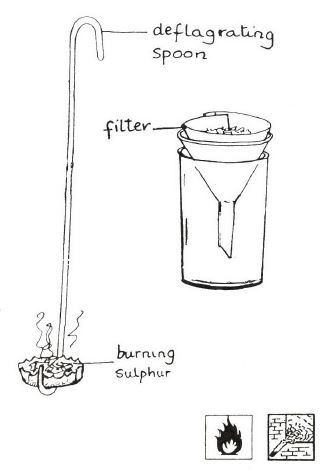
\includegraphics[width=0.28\textwidth]{./img/source/sulphur-monoclinic.jpg}
\end{center}

\begin{description*}
%\item[Subtopic:]{}
\item[Materials:]{Powdered sulphur, bottle cap, candle, paper funnel, deflagrating spoon, bottle}
%\item[Setup:]{}
\item[Procedure:]{Put 3-4 spatulas of powdered sulphur into a
bottle top. Heat very
gently until it is just melted or plasticised. Pour the
molten sulphur, which should be a clear yellow
liquid, into a filter paper funnel. Leave
to cool until a crust just forms on the
surface of the sulphur. Break open the surface to
expose the crystals underneath.}
\item[Hazards:]{Sulphur can catch fire to produce noxious
fumes of sulphur dioxide.}
%\item[Questions:]{}
\item[Observations:]{Thin needle-like crystals of monoclinic
sulphur are seen.}
\item[Theory:]{Sulphur has two allotropes, rhombic and
monoclinic sulphur. Rhombic sulphur is the
more stable form. The transition temperature
between the two is 96$^\circ$C. Since sulphur
melts at 116$^\circ$C, melting and
allowing it to cool slightly exceeds the transition
temperature and monoclinic sulphur
is formed. It will revert to its
more stable form, rhombic sulphur, in a few
days time.}
%\item[Applications:]{}
%\item[Notes:]{}
\end{description*}

\subsection{Reaction of Sulphur with \hfill \\ Metals} % LASM 139

%\begin{center}
%\includegraphics[width=0.4\textwidth]{./img/.jpg}
%\end{center}

\begin{description*}
%\item[Subtopic:]{}
\item[Materials:]{Sulphur powder, copper wire, two spoons, \nameref{sec:heatsources}, scissors, match box}
%\item[Setup:]{}
\item[Procedure:]{Cut the copper wire into small pieces and place a few onto a spoon. Add a small amount of sulphur and mix (there should be more sulphur than copper). Heat the mixture over a flame until it turns black.}
\item[Hazards:]{This reaction produces sulphur dioxide, a poisonous gas. Perform outside or in a well-ventilated room and stand upwind.}
%\item[Questions:]{}
%\item[Observations:]{}
\item[Theory:]{Copper and sulphur react to form black copper (II) sulphide.}
%\item[Applications:]{}
%\item[Notes:]{}
\end{description*}

\columnbreak

%==================================================================================================%

\section*{Sulphur Dioxide}


\subsection{Production of Sulphur Dioxide Gas} % VSO 67, Source 170

\begin{center}
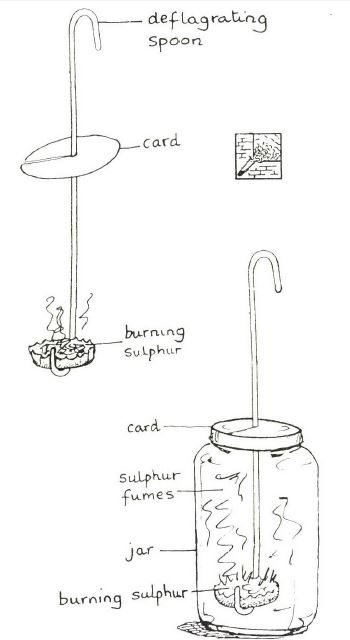
\includegraphics[width=0.4\textwidth]{./img/source/sulphur-dioxide.jpg}
\end{center}

\begin{description*}
%\item[Subtopic:]{}
\item[Materials:]{Cardboard/manila, deflagrating spoon, sulphur, bottle cap, jar, candle}
%\item[Setup:]{}
\item[Procedure:]{Cut out a circle of stiff paper or cardboard and
fix it onto the deflagrating spoon as shown in the
diagram. Put 2-3 spatulas of sulphur into a bottle
top and heat it in a flame until the sulphur
catches fire. Immediately transfer the
deflagrating spoon into a glass jar.}
\item[Hazards:]{Sulphur dioxide fumes are noxious, thus
experiment should be done in a well ventilated
room, near an open window or in a fume
chamber.}
%\item[Questions:]{}
\item[Observations:]{The sulphurburns with a blue flame. Choking
fumes of gas are produced.}
\item[Theory:]{Sulphur burns in air to form choking fumes
of sulphur dioxide gas.}
%\item[Applications:]{}
%\item[Notes:]{}
\end{description*}

\subsection{Sulphuric Acid}

\begin{center}
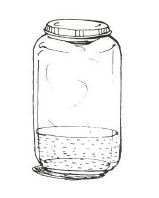
\includegraphics[width=0.3\textwidth]{./img/source/sulphuric-acid.jpg}
\end{center}

\begin{description*}
%\item[Subtopic:]{}
\item[Materials:]{Jar of sulphur dioxide gas, indicator, water}
%\item[Setup:]{}
\item[Procedure:]{Add water to the jar of sulphur dioxide gas and
then add some indicator.}
%\item[Hazards:]{}
%\item[Questions:]{}
\item[Observations:]{The gas dissolves and the solution is acidic
(the universal indicator paper turns red).}
\item[Theory:]{Sulphur dioxide gas is very soluble in water.
It forms an acidic solution called sulphuric (IV)
acid. }
\item[Applications:]{This is the principle on which acid rain is
formed.}
%\item[Notes:]{}
\end{description*}

\subsection{Bleaching Effects of Sulphur Dioxide}

\begin{center}
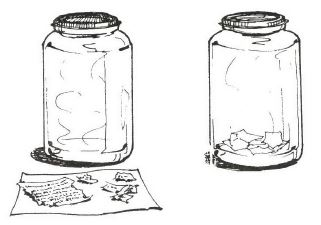
\includegraphics[width=0.4\textwidth]{./img/source/sulphur-dioxide-bleaching.jpg}
\end{center}

\begin{description*}
%\item[Subtopic:]{}
\item[Materials:]{Jar of sulphur dioxide gas, newspaper}
%\item[Setup:]{}
\item[Procedure:]{To a jar of sulphur dioxide gas add a small
piece of a newspaper. Firmly replace the lid of
the jar.}
\item[Hazards:]{This reaction produces sulphur dioxide, a poisonous gas. Perform this
reaction outside or in a well-ventilated room and stand upwind.}
%\item[Questions:]{}
\item[Observations:]{The newspaper is bleached.}
\item[Theory:]{Sulphur dioxide gas is a bleaching agent.
This experiment works well when the sulphur
dioxide gas is in high concentration.}
%\item[Applications:]{}
%\item[Notes:]{}
\end{description*}

\columnbreak

%\subsection{Acid Rain}
%
%\begin{center}
%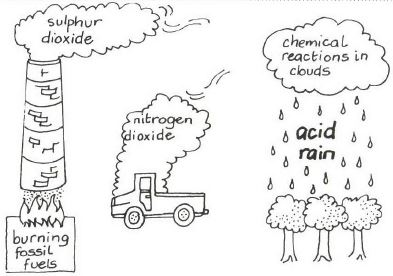
\includegraphics[width=0.45\textwidth]{./img/vso/acid-rain.jpg}
%\end{center}
%
%\begin{description*}
%%\item[Subtopic:]{}
%%\item[Materials:]{}
%%\item[Setup:]{}
%%\item[Procedure:]{}
%%\item[Hazards:]{}
%%\item[Questions:]{}
%%\item[Observations:]{}
%\item[Theory:]{The above diagram shows how acid rain
%forms when sulphur dioxide and other gases
%react with rain water.}
%%\item[Applications:]{}
%%\item[Notes:]{}
%\end{description*}

%==================================================================================================%

\section*{Nitrogen}


\subsection{Sources of Nitrogen}

\begin{center}
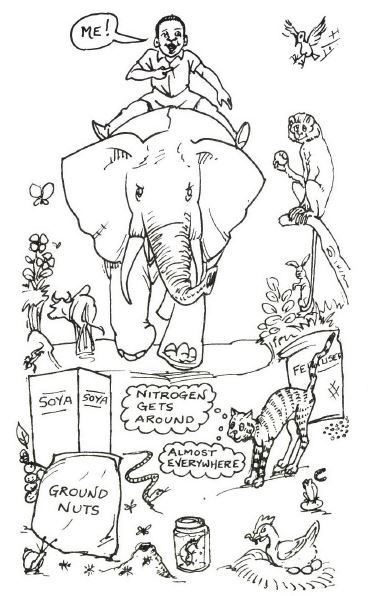
\includegraphics[width=0.49\textwidth]{./img/source/nitrogen-sources.jpg}
\end{center}

\begin{description*}
%\item[Subtopic:]{}
%\item[Materials:]{}
%\item[Setup:]{}
\item[Procedure:]{Make a display (or prepare wall
charts) of\\
(a) food rich in proteins, e.g. fish, meat;\\
(b) nitrogen fertilizers;\\
(c) soldering stone (\ce{NH4Cl}) as used by welders.\\
All plants contain a certain amount of protein,
but some have a high concentration, particularly
seeds like cow pea, groundnut and soya bean.}
%\item[Hazards:]{}
%\item[Questions:]{}
%\item[Observations:]{}
%\item[Theory:]{}
%\item[Applications:]{}
%\item[Notes:]{}
\end{description*}

%\vfill
%\columnbreak

\end{multicols}

\subsection{Preparation of Nitrogen Gas} % LASM

\begin{center}
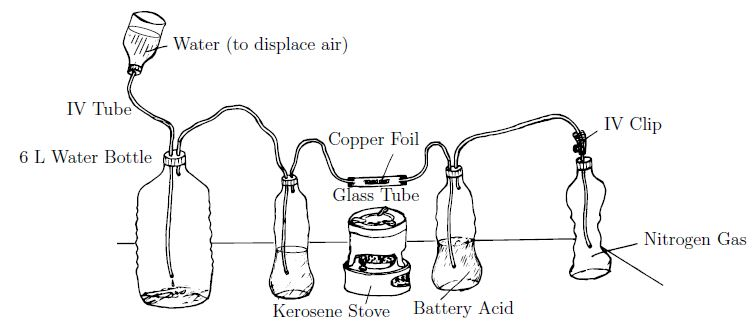
\includegraphics[width=0.9\textwidth]{./img/nitrogen-gas.png}
\end{center}

%\columnbreak
\begin{multicols}{2}

\begin{description*}
%\item[Subtopic:]{}
\item[Materials:]{Large water bottle (6 L), caustic soda (sodium hydroxide), battery acid (5 M
sulphuric acid), delivery tubes, \nameref{sec:heatsources}, piece of glass tube (about 20
cm), 4 empty water bottles (1 or 1.5 L), very thin copper wire}
\item[Setup:]{Poke 2 holes in each of 2 bottle tops; in the third top poke 1 hole. Connect the delivery tubes in these holes using pen tubes as
junctions Insert the copper turnings inside the glass tube. Prepare a 2 M solution of caustic soda in a 1~L bottle with two holes in the cap. Put sulphuric acid in the other bottle with two holes in the cap.
Arrange the apparatus set up as in the figure making sure that the last
bottle is squeezed (compressed) to remove air before collection.}
\item[Procedure:]{Add water through the funnel into the 6 L bottle so as to displace air
present in the bottle. This is done after the copper turning starts
to be red hot. Observe what happens in the two water bottles A and B as well as the
changes of the red hot copper turning in the combustion tube. 
%\columnbreak
Observe the expansion of the bottle C as water fills the 6 L bottle. Collect the gas in the bottle C by tightening the delivery tube.}
\item[Hazards:]{Sodium hydroxide (caustic soda) is corrosive to the skin and even in a
dilute solution can blind. Avoid contact with skin and eyes. Neutralize
spills with citric acid solution. Concentrated sulphuric acid is
corrosive to the skin and clothes. Avoid contact with skin and eyes.
Neutralize spills with bicarbonate of sodium (baking soda).}
%\item[Questions:]{}
\item[Observations:]{Copper turnings turn red hot when heated in the absence of air (i.e. before
water is added to the 6 L bottle. After the addition of water to 6 L bottle,
bubbles will be observed in both A and B and the red hot copper turnings
turn black. }
\item[Theory:]{The collection bottle (C) should expand. The black colour of
copper indicates oxidation of copper by atmospheric oxygen. Copper oxide
is black. The bubbles observed in the bottles indicates the passage of air into
the solution.}
%\item[Applications:]{}
%\item[Notes:]{}
\end{description*}

\subsection{Nitrogen Oxides from \hfill \\ Lightning}

\begin{center}
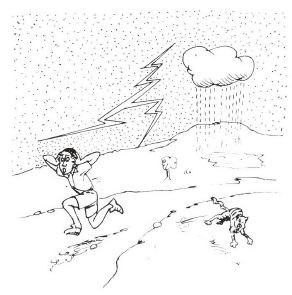
\includegraphics[width=0.49\textwidth]{./img/source/nitrogen-lightning-2.jpg}
\end{center}

\begin{description*}
%\item[Subtopic:]{}
%\item[Materials:]{}
%\item[Setup:]{}
%\item[Procedure:]{}
%\item[Hazards:]{}
%\item[Questions:]{}
%\item[Observations:]{}
\item[Theory:]{During thunderstorms, lightning heats
the air locally to a very high temperature. Thus
nitrogen and oxygen from the air react to form
nitrogen oxides. Some of these are converted by
further reaction with rain water to nitric acid
which in the soil forms nitrates. The latter are
nitrogen fertilizers. Hence, if the pollutants
from vehicles are absent,
thunderstorms contribute to the fertilization of
fields in this way.}
%\item[Applications:]{}
%\item[Notes:]{}
\end{description*}

\columnbreak

\subsection{Nitrogen Circulation}

\begin{center}
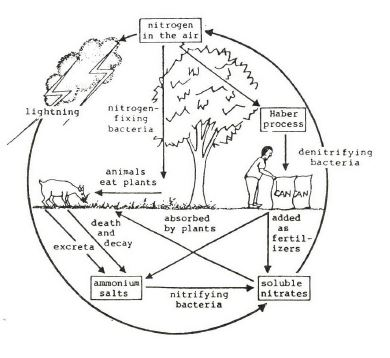
\includegraphics[width=0.49\textwidth]{./img/source/nitrogen-cycle.jpg}
\end{center}

\begin{description*}
%\item[Subtopic:]{}
\item[Materials:]{Cards/manila, flip chart}
%\item[Setup:]{}
\item[Procedure:]{Prepare a wall chart of the natural nitrogen
circulation or make cards of the various steps for students to place. }
%\item[Hazards:]{}
%\item[Questions:]{}
%\item[Observations:]{}
\item[Theory:]{When proteins are broken down in
the body, combined nitrogen containing
compounds leave the body with the urine. These
compounds are broken down further by bacteria
to ammonia (NH$_4$) which makes for example
public places of urination smell very badly.
Dead plant and animal tissues are similarly
broken down. The ammonia formed is washed
into the soil, where it is acted upon by different
types of bacteria, eventually converting it into
nitrates and ammonium salts which are needed
by plants to produce proteins. Hence they are
important fertilizers.}
%\item[Applications:]{}
%\item[Notes:]{}
\end{description*}

\vfill
\columnbreak

%==================================================================================================%

\section*{Ammonia}


\subsection{Preparation of Ammonia Gas} % Source 164, LASM

\begin{center}
%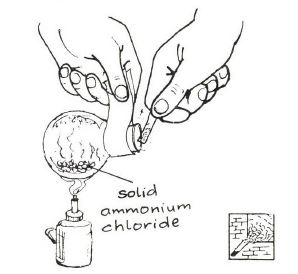
\includegraphics[width=0.4\textwidth]{./img/source/ammonia.jpg}
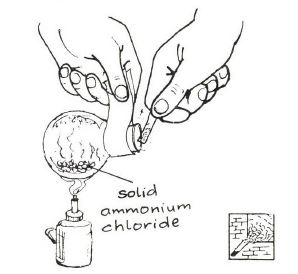
\includegraphics[width=0.45\textwidth]{./img/source/ammonia.jpg}
\end{center}

\begin{description*}
%\item[Subtopic:]{}
\item[Materials:]{Ammonium sulphate, caustic soda (sodium hydroxide),
red litmus paper, match box, conc. HCl (optional), \nameref{sec:heatsources}, heating
vessel}
\item[Setup:]{Prepare sodium hydroxide solution by dissolving approximately 1 spoon of
sodium hydroxide in about 200 mL of water.}
\item[Procedure:]{Put one tea spoon of ammonium sulphate into a heating vessel. Add about 100 mL of sodium hydroxide solution to the ammonium
sulphate and mix. Warm the mixture using a heat source. Test the gas evolved using moist red litmus paper. Record observations and note the smell of the gas.

\emph{Optional}: Bring a bottle containing conc. HCl acid, open it and allow
fumes coming out of the bottle to react with the gas evolved from the
gas generator.}
%\item[Hazards:]{}
%\item[Questions:]{}
\item[Observations:]{Ammonia is a colourless gas with pungent smell (smell of urine), it turns red
litmus blue. It also forms white fumes when it comes into contact with HCl
vapors.}
\item[Theory:]{Ammonia gas is the only alkaline gas known, it reacts with hydrogen
chloride gas to form thick/dense white fumes of ammonium chloride (This
is the identification of the gas). It is highly soluble in water, which is why
it can't be collected over water. It is less dense than air that is why it is
collected by downward displacement of air (upward delivery).}
%\item[Applications:]{}
%\item[Notes:]{}
\end{description*}

\vfill
\columnbreak

%==================================================================================================%

\section*{Carbon Dioxide}


\subsection{Production of Carbon \hfill \\ Dioxide Gas} % Shika 283(A), Source 70

\begin{center}
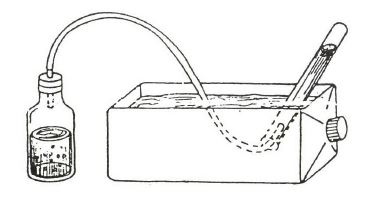
\includegraphics[width=0.4\textwidth]{./img/source/co2-generator.jpg}
\end{center}

\begin{description*}
%\item[Subtopic:]{}
\item[Materials:]{Plastic bottle, plastic tube, syringe, wood ash, dilute acid (e.g. citric acid)}
%\item[Setup:]{}
\item[Procedure:]{Assemble the apparatus as shown. Put a
spoonful of ash into the bottle, add some dilute
acid and close the bottle
immediately. The syringe fills with gas.}
%\item[Hazards:]{}
%\item[Questions:]{}
%\item[Observations:]{}
\item[Theory:]{The potassium carbonate in wood ash reacts
with dilute acid to produce carbon dioxide gas.}
%\item[Applications:]{}
%\item[Notes:]{}
\end{description*}

\subsection{\textbf{CO}$_\textbf{2}$ Balloon}

\begin{center}
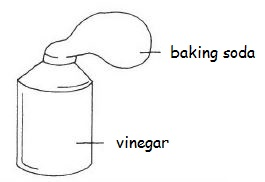
\includegraphics[width=0.35\textwidth]{./img/vso/co2-balloon.jpg}
\end{center}

\begin{description*}
%\item[Subtopic:]{}
\item[Materials:]{Bottle, baking soda, vinegar, balloon}
%\item[Setup:]{}
\item[Procedure:]{Add a small amount of vinegar into a bottle. Fill a balloon with baking soda (bicarbonate of soda) and stretch the balloon over the mouth of the bottle. Lift the balloon to empty the contents into the bottle.}
%\item[Hazards:]{}
%\item[Questions:]{}
\item[Observations:]{The balloon fills up with gas and may even explode!}
\item[Theory:]{The vinegar and baking soda combine to produce carbon dioxide gas, which gets collected in the balloon.}
\item[Applications:]{Employ the scientific method by varying the concentrations of vinegar and baking soda to see the effect on the amount of CO$_2$ gas released.}
%\item[Notes:]{}
\end{description*}

\subsection{Test for Carbon Dioxide}

\begin{center}
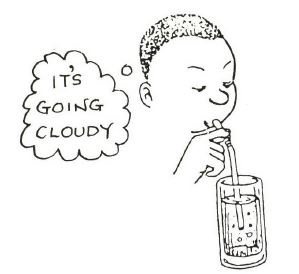
\includegraphics[width=0.4\textwidth]{./img/source/limewater-cloudy.jpg}
\end{center}

\begin{description*}
%\item[Subtopic:]{}
\item[Materials:]{Bottle, lime water, straw}
%\item[Setup:]{}
\item[Procedure:]{Pour some lime water into a bottle and blow (with
a straw or a tube) bubbles of air into lime water. It will take
some time until you can observe a change.}
%\item[Hazards:]{}
%\item[Questions:]{}
\item[Observations:]{The lime water becomes cloudy, proving the presence of carbon dioxide in our exhaled air.}
%\item[Theory:]{}
%\item[Applications:]{}
%\item[Notes:]{}
\end{description*}

\subsection{\textbf{CO}$_\textbf{2}$ in Soda} % Shika 294 (Combine all)

%\begin{center}
%\includegraphics[width=0.4\textwidth]{./img/.jpg}
%\end{center}

\begin{description*}
%\item[Subtopic:]{}
\item[Materials:]{Unopened soda bottle}
%\item[Setup:]{}
\item[Procedure:]{(a) Open the soda bottle and watch how long it takes to stop releasing carbon dioxide (when bubbles stop forming). (b) Repeat but first shake the soda bottle before opening. (c) Repeat again but add salt after the initial carbon dioxide has escaped. }
%\item[Hazards:]{}
%\item[Questions:]{}
\item[Observations:]{The soda in part (b) is sprayed out of the bottle at a high pressure. In part (c), adding salt helps to remove the remaining carbon dioxide in the soda.}
\item[Theory:]{When soda is bottled, CO$_2$ gas is pumped in at high pressure, and some of it dissolves in the soda. Removing the top allows this pressurized gas to escape, although some of the CO$_2$ remains attracted to water molecules. This is why carbonation remains for some time after opening. 

Shaking the bottle causes previously escaped CO$_2$ to redissolve in the soda and form large bubbles which rush to the surface to escape the solution.

Water has a greater attraction to the salt molecules than the CO$_2$ molecules, so adding salt causes the water to release the CO$_2$ molecules and push them together. They combine and form larger bubbles, which rise to the surface of the soda.}
%\item[Applications:]{}
%\item[Notes:]{}
\end{description*}



\end{multicols}

\pagebreak